\documentclass[handout]{beamer}
\usetheme{focus}
\usepackage{graphicx}
\usepackage{svg}
\usepackage{amssymb,amsmath}
\usepackage{dsfont}
\usepackage{caption}
\usepackage{subcaption}

\title{Graph eigenvectors estimation by random walk and diffusion}
\subtitle{A study of robustness}
\author{Hoang NT}
\titlegraphic{
\includegraphics[scale=0.12]{imgs/spectrahedron.png}}
\institute{Murata Laboratory \\ Tokyo Tech \vspace{4em}}
\date{2018/10/24}

\begin{document}
    \begin{frame}
        \maketitle
    \end{frame}

    \begin{frame}{Overview}
        \tableofcontents
    \end{frame}
    
    \section{Stability problem}

    \subsection{Observation}

    \begin{frame}{Eigen-mass shift}
        Consider a "basically expander" graph G, except that it has two poorly connected components:
        \begin{figure}
            \centering
            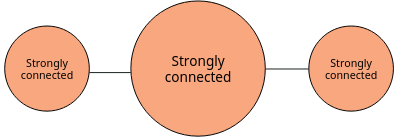
\includegraphics[scale=0.5]{imgs/ex1_graph_unstable.png}
            \caption{Almost expander graph.}
            \label{fig:ex1_G_unstable}
        \end{figure}
        \pause
        The problem with this kind of graph is: It is easy to change the edge weights of the central part to make the "mass" of the leading non-trivial eigenvector on the first small component or the second component. \pause \textbf{Stability of eigendirection} is clearly an issue. 

    \end{frame}
    \begin{frame}{Example}
        Graph $G$ having 13 nodes, by removing edge (0,1) we get $G'$:
        \begin{figure}
        \centering
        \begin{subfigure}{.5\textwidth}
          \centering
          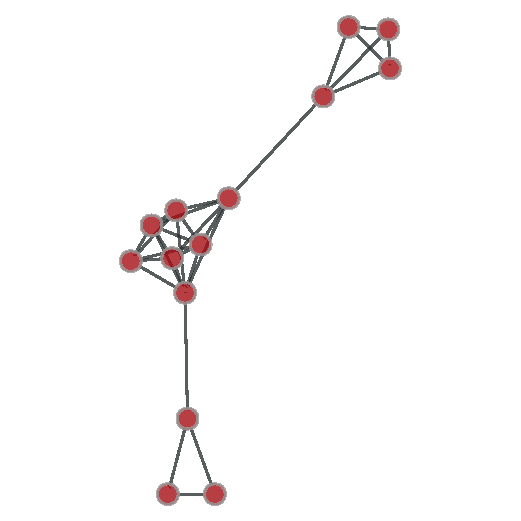
\includegraphics[width=.45\linewidth]{imgs/ex2_graph_13_full.pdf}
          \caption{Original graph ($G$)}
          \label{fig:ex2_graph_full}
        \end{subfigure}%
        \begin{subfigure}{.5\textwidth}
          \centering
          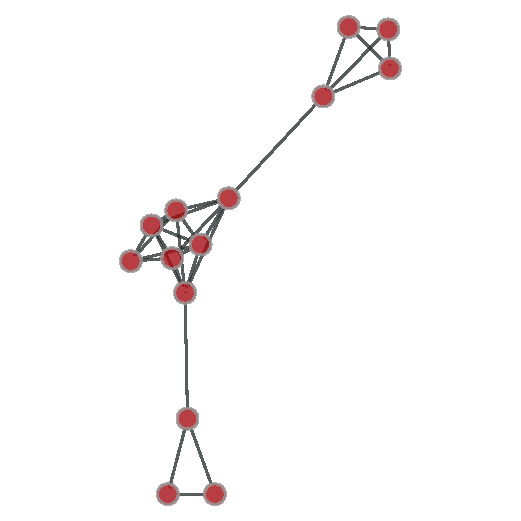
\includegraphics[width=.45\linewidth]{imgs/ex2_graph_13.pdf}
          \caption{Perturbed graph ($G'$)}
          \label{fig:ex2_graph_pert}
        \end{subfigure}
        \caption{Almost expander graphs.}
        \label{fig:ex2}
        \end{figure}
        The two first non-trivial eigenvectors of these graphs are:
        \tiny
        \begin{align*}
        v^G_1 &= 
             \begin{bmatrix} 
                -0.208 & -0.286 & -0.275 & -0.275 & -0.275 & -0.212 & -0.275 & 0.225 & 0.394 & 0.395 & 0.126 &  0.221 &  0.221 & 0.221 
             \end{bmatrix} \\            
        v^{G'}_1 &= 
             \begin{bmatrix} 
                0.194 & 0.307 & 0.275 & 0.275 & 0.275 & 0.208 & 0.275 & -0.224 & -0.387 & -0.387 & -0.131 & -0.226 & -0.226 & -0.226
             \end{bmatrix} \\
        \end{align*}
    \end{frame}

    \begin{frame}{Similar problem in Linear Program}
        Consider an optimization problem:
        $$ \min_{x \in \mathcal{S}} f(x) $$
        \pause
        This problem might not be "well-posed", so we add a \textit{regularization} term $\lambda g(x)$:
        $$ \min_{x \in \mathcal{S}} f(x) + \lambda g(x) $$
        \pause
        If we choose $g(x)$ to be strongly convex ($\sigma$-strongly convex), we can obtain: increased stability; \pause decreased sensitivity to noise; \pause and avoid overfitting.
    \end{frame}

    \subsection{Effectiveness of approximation methods}
    \begin{frame}{Practical approximation methods}
    In theory, eigenvectors provide a nice way for graph analysis. \pause However, spectral clustering methods are usually worse than heuristic/approximation-based methods \cite{perozzi2014deepwalk,leskovec2008statistical}.\linebreak
    \\
    \pause
    \noindent
    Hence, there must be some form of \textbf{implicit} regularization for each of these heuristic algorithms.
        \begin{block}{Research question}
            To what extent can one formaliza the idea that performing an approximate computation can implicitly lead to more regular solutions? \cite{mahoney2010implementing}. \vspace{0.5em}
        \end{block}
    \end{frame}

    \section{Implicit regularizations}

    \subsection{Problem definition}

    \begin{frame}{Aim}
        The aim of paper \cite{mahoney2010implementing} is to connect the solution of a regularized SDP problem to three diffrent commonly used random walk heuristics:
        \begin{description}
        \item[Heat Kernel]
        An operator describing the diffusive spreading of heat on the graph.
        $$ H_t = \exp{(-tL)} = \sum_{k=0}^{\inf} \frac{(-t)^k}{k!}L^k $$
        \pause
        \item[PageRank]
        The PageRank vector is given by:
        $$ \pi(\gamma, s) = \gamma s + (1-\gamma)M\pi(\gamma,s) $$
        \pause
        \item[TLRW]
        $M = AD^{-1}$ is the natural random walk transition matrix, the Truncated $\alpha$-Lazy Random Walk matrix is given by:
        $$ W_\alpha = \alpha I + (1-\alpha)M $$
        \end{description}
    \end{frame}

    \begin{frame}{SPECTRAL problem}
        \pause
        Consider the standard SPECTRAL problem:
        \begin{equation*}
            \begin{array}{ll@{}ll}
            \text{min} & x^TLx \\
            \text{s.t.}& x^Tx = 1\\
                       & x^TD^{1/2}1 = 0
            \end{array}
        \end{equation*}
        \pause
        This problem is \textit{equivalent} to a SDP:
        \begin{equation*}
            \begin{array}{ll@{}ll}
            \text{min} & L \cdot X \\
            \text{s.t.}& Tr(X) = I \cdot X = 1\\
                       & X \succeq 0
            \end{array}
        \end{equation*}
        \pause
    The exact solution for SDP is when $X$ is rank-1, i.e. $X=xx^T$. However, when the solution is not rank-1, a simple way to construct a vector $x$ from $X$ is to sample $\xi \backsim N(0,1/n)$ and build $x = X^{1/2} \xi$.
    \end{frame}
    
    \begin{frame}{Regularized SDP}
        Consider the form:
        \begin{equation*}
            \begin{array}{ll@{}ll}
            (F,\eta) - SDP & \text{min} & L \cdot X + \frac{1}{\eta} F(X) \\
                           & \text{s.t.}& I \cdot X = 1\\
                           &            & X \succeq 0
            \end{array}
        \end{equation*}

        The authors of \cite{mahoney2010implementing} connects the regularization term $F(X)$ and approximation heuristic as follow:
        \pause
        \begin{itemize}
        \item When $F(X)$ is \textbf{von Neumann entropy}, the solution $X^{\ast}$ can be obtained by the \textbf{heat kernel}.
        \pause
        \item When $F(X)$ is \textbf{log-determinant}, the solution $X^{\ast}$ can be obtained by \textbf{PageRank}.
        \pause
        \item When $F(X)$ is \textbf{matrix p-norm}, the solution $X^{\ast}$ can be obtained by \textbf{truncated lazy random walk}.
        \end{itemize}
    \end{frame}

    \subsection{Solution to the regularized SPD}
    
    \begin{frame}{Solution to the regularized SPD}
        \begin{block}{Theorem 1 \cite{mahoney2010implementing}\vspace{0.5em}}
        Let $G$ be a connected, weighted, undirected graph, with normalized Laplacian $L$. Then, the following conditions are sufficient for $X^\ast$ to be an optimal solution to $(F,\eta) - SDP$.
        \begin{enumerate}
            \item $X^\ast = (\nabla F)^{-1}(\eta(\lambda^\ast I - L)), \text{for } \lambda^\ast \in \mathds{R}$,
            \item $I \cdot X^\ast = 1$,
            \item $X^\ast \succeq 0$.
        \end{enumerate}
        \vspace{0.5em}
        \end{block}
    \end{frame}

    \begin{frame}{Proof of theorem 1}
        \pause
        The proof is pretty straight-forward. Write the Lagrangian $\mathcal{L}$ as:        $$\mathcal{L} = L \cdot X + \frac{1}{\eta} \cdot F(X) - \lambda \cdot (I \cdot X - 1) - U \cdot X$$
        \pause
        Set the gradient of the Lagrangian w.r.t. X to 0:
        $$\nabla \mathcal{L} = L + \frac{1}{\eta}(\nabla F)X-\lambda I - U = 0 $$
        \pause
        The dual objective function is minimized when:
        $$X = (\nabla F)^{-1} (\eta (-L + \lambda^\ast I + U))$$
        \pause
        We choose $\lambda^\ast$ to satisfy the second condition. By Weak Duality ( primal problem solution is always greater than or equal to an associated dual problem solution), $X^\ast$ ($X$ with appropriate $\lambda^\ast$) is an optimal solution to $(F,\eta) - SDP$.
    \end{frame}

    \subsection{Plug the regularizer in!}
    
    \begin{frame}{Generalized Entropy and the Heat Kernel}
        \pause
        The generalized entropy function (also von Neumann entropy):
        $$F_H(X) = Tr(X \log{X}) - Tr(X) $$
        \pause
        for which:
        \begin{align*}
        (\nabla F_H)(X) &= \log{X}\\            
        (\nabla F_H)^{-1}(Y) &= \exp{Y}.
        \end{align*}
        \pause
        Hence, the solution to $(F_H,\eta) - SDP$ is:
        $$X^\ast_H = \exp{(\eta (\lambda I - L)}$$
        \pause
        By setting $\lambda = -1/\eta \log{(Tr(exp(-\eta L)))}$, we have:
        $$X*\ast_H = \frac{H_\eta}{Tr(H_\eta)}$$.
    \end{frame}
    
    \begin{frame}{Log-determinant and PageRank}
        The log-determinant function is given by:
        $$F_D(X) = -\log{\det{X}}$$
        Similar to the previous manipulation, lemma 2 of \cite{mahoney2010implementing} showed that:
        $$X^\ast_D = \frac{D^{-1/2} R_\gamma D^{-1/2}}{Tr(R_\gamma)}$$
    \end{frame}

    \begin{frame}{p-norm and Truncated Lazy Random Walk}
        The p-norm function is given by:
        $$F_p(X) = \frac{1}{p} \parallel X \parallel^p_p = \frac{1}{p} Tr(X^p)$$
        Lemma 3 of \cite{mahoney2010implementing} showed that:
        $$X^\ast_p = \frac{D^{\frac{-(q-1)}{2}W_\alpha^{q-1}D^{\frac{q-1}{2}}}}{Tr(W_\alpha^{q-1})}$$
        Thus connecting the p-norm and the heuristic algorithms on TLRW matrix.
    \end{frame}
    
    \section{Conclusion}

    \subsection{Summary}
    \begin{frame}{Summary}
        \begin{figure}
            \centering
            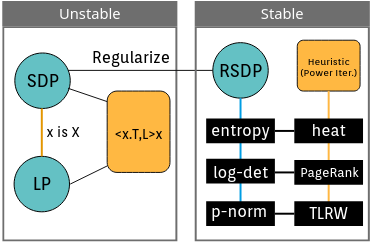
\includegraphics[scale=0.7]{imgs/sum.png}
            \caption{Graphical summary.}
            \label{fig:sum}
        \end{figure}
    \end{frame}

    \subsection{Discussion}
    \begin{frame}{Discussion}
        The random-walk-based (also difussion-based) view provided several benefits:        \begin{itemize}
        \item Robustness and stability in computation 
        \item Insight on how heuristic algorithms worked better than spectral methods.
        \end{itemize}
    \end{frame}
    
    \appendix
    \begin{frame}{References}
        \nocite{*}
        \bibliography{main}
        \bibliographystyle{plain}
    \end{frame}
\end{document}
